\documentclass{article}
\usepackage[T1]{fontenc}
\usepackage{lmodern}
\usepackage{graphicx}
\usepackage{amsmath,amssymb}
\usepackage[a4paper,margin=2cm]{geometry}
\usepackage[absolute,overlay]{textpos}
\setlength{\TPHorizModule}{1mm}
\setlength{\TPVertModule}{1mm}
\usepackage[indonesian]{babel}
\usepackage{hyperref}
\setlength{\emergencystretch}{2em}
% unit: Halaman 14

\begin{document}

% === Halaman 14 (llm) ===

\vspace{237.60mm}

Demo kalkulkator ECC online: \url{https://andrea.corbellini.name/ecc/interactive/reals-add.html}

\vspace{10mm}

Point addition over the elliptic curve \[ y^2 = x^3 - 7x + 10 \] in $\mathbb{R}$.

% deskripsi: Tangkapan layar kalkulator interaktif Elliptic Curve point addition yang menunjukkan grafik kurva eliptik, garis yang menghubungkan titik P dan Q, serta input parameter kurva dan koordinat titik-titiknya.
% bbox normalisasi: [0.0400, 0.1600, 0.9500, 0.9600]
\begin{textblock*}{191.10mm}(8.40mm,47.52mm)
\noindent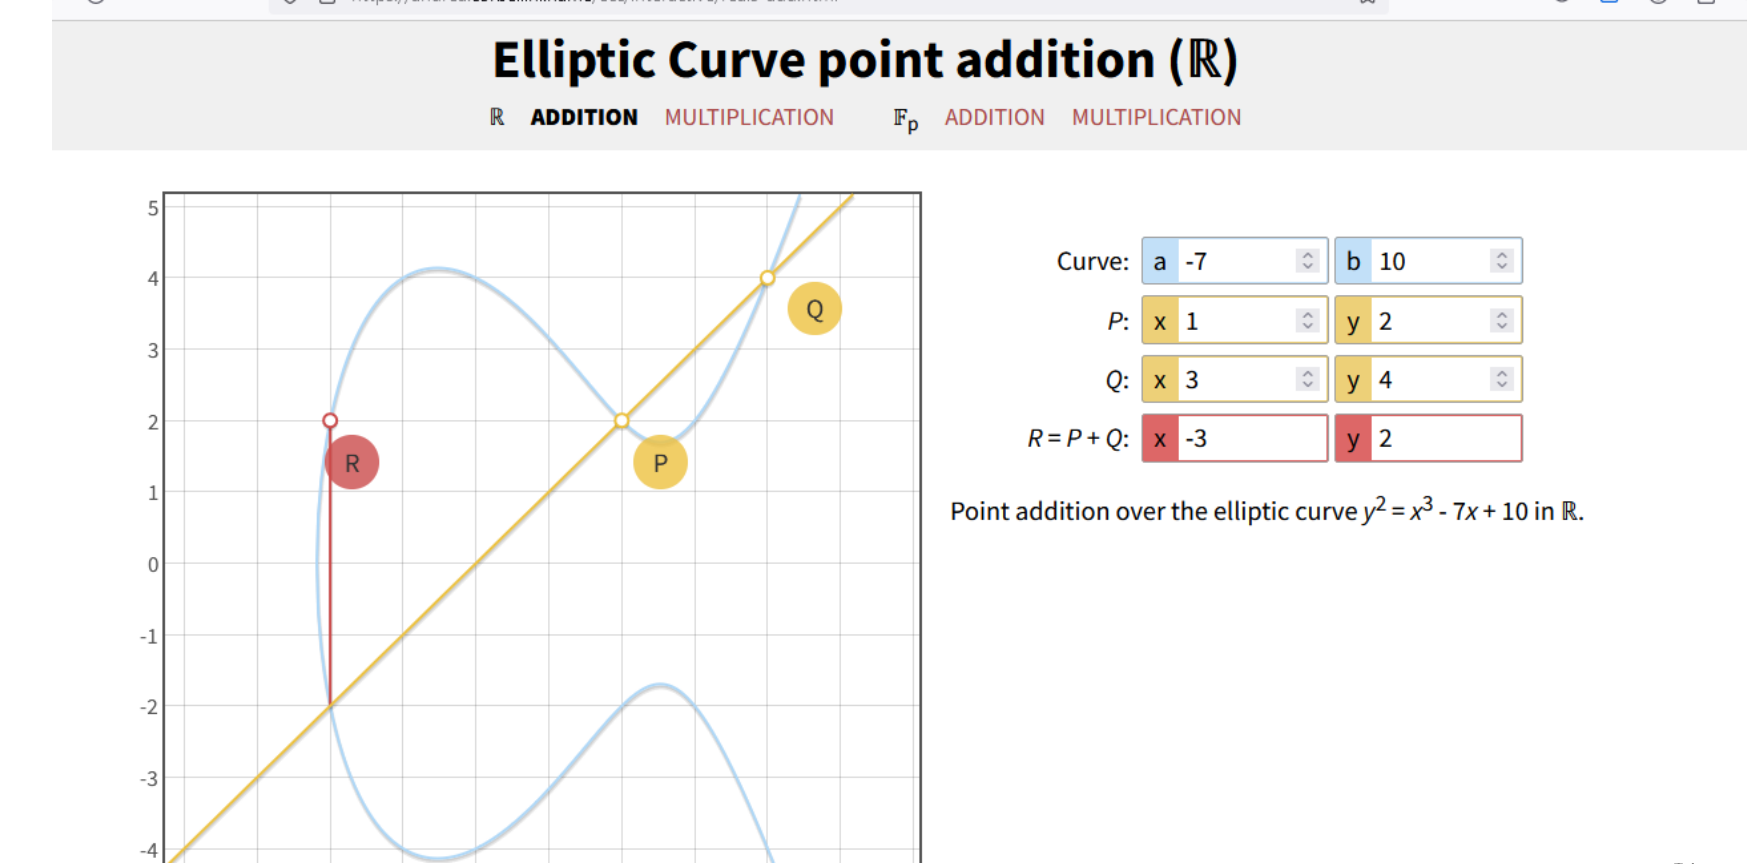
\includegraphics[width=191.10mm,height=237.60mm]{../../images/llm/page_014_img_01.png}%
\end{textblock*}

\end{document}
